
\begin{figure}
	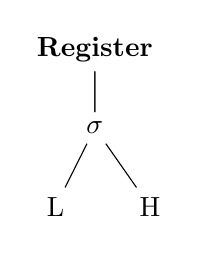
\begin{tikzpicture}	
		\node (tbu) at (.5,0) {\textbf{Register}};
		\node (R) at (.5,-1) {$\sigma$};
		\node (r1) at (0,-2) {L};
		\node (r2) at (1.2,-2) {H};
		\draw (tbu) -> (R) -> (r1);
		\draw (tbu) -> (R) -> (r2);
	\end{tikzpicture}
	\hfill
	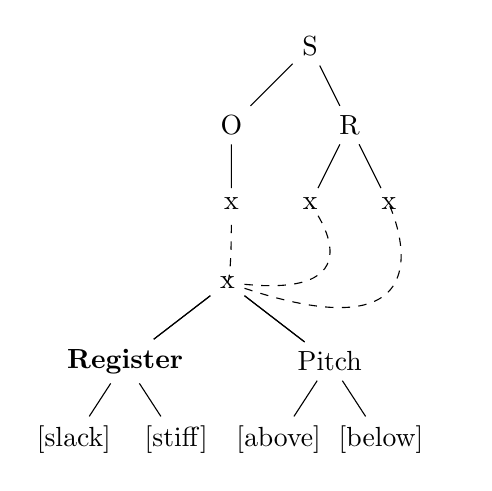
\begin{tikzpicture}
		\node (tbu) at (1.95,0) {x};
		\node (R) at (.65,-1) {\textbf{Register}};
		\node (P) at (3.25,-1) {Pitch};
		\node (r1) at (0,-2) {[slack]};
		\node (r2) at (1.3,-2) {[stiff]};
		\node (p1) at (2.6,-2) {[above]};
		\node (p2) at (3.9,-2) {[below]};
		\draw (tbu) -> (R) -> (r1);
		\draw (tbu) -> (R) -> (r2);
		\draw (tbu) -> (P) -> (p1);
		\draw (tbu) -> (P) -> (p2);
		% Second graph (shifted right)
		\begin{scope}[xshift=3cm, yshift=3cm]
			\node (sS) at (0,0) {S};
			\node (o) at (-1,-1) {O};
			\node (r) at (0.5,-1) {R};
			\node (x1) at (-1,-2) {x};
			\node (x2) at (0,-2) {x};
			\node (x3) at (1,-2) {x};
			\draw (sS) -> (o) -> (x1);
			\draw (sS) -> (r) -> (x2);
			\draw (r) -> (x3);
		\end{scope}
		
		% Cross edges from TBU to Xs
		\draw[dashed] (tbu) .. controls +(0,0) and +(0,-1) .. (x1);
		\draw[dashed] (tbu) .. controls +(2,-0.2) and +(0,0) .. (x2);
		\draw[dashed] (tbu) .. controls +(3,-1) and +(0,0) .. (x3);
	\end{tikzpicture}
	\hfill
	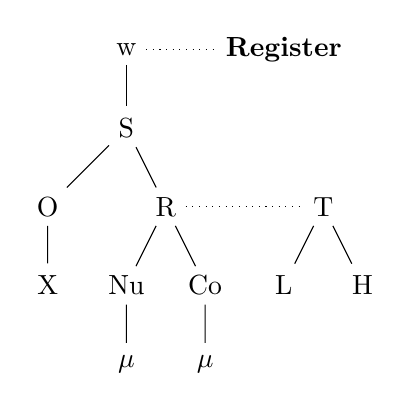
\begin{tikzpicture}[-,shorten >=1pt]
		\tikzstyle{state}=[fill=white,draw=black,text=black,node distance=16mm]
		
		\node (w) at (0,1) {w};
		\node (re) at (2,1) {\textbf{Register}};
		\node (s) at (0,0) {S};
		\node (o) at (-1,-1) {O};
		\node (r) at (0.5,-1) {R};
		\node (T) at (2.5,-1) {T};
		\node (t1) at (2.0,-2) {L};
		\node (t2) at (3,-2) {H};
		
		\node (x1) at (-1,-2) {X};
		\node (x2) at (0,-2) {Nu};
		\node (x3) at (1,-2) {Co};
		\node (m1) at (0,-3) {$\mu$};
		\node (m2) at (1,-3) {$\mu$};
		\draw (w) -> (s);
		\draw (T) -> (t1);
		\draw (T) -> (t2);
		\draw (s) -> (o) -> (x1) ;
		\draw (s) -> (r) -> (x2) -> (m1);
		\draw (r) -> (x3) -> (m2);
		\draw [dotted](r) -> (T);
		\draw [dotted](w) -> (re);
	\end{tikzpicture}
	\label{three-rep}
\end{figure}
